%---------------------------------------------------------------------
%
%                          Cap�tulo 1
%
%---------------------------------------------------------------------

\chapter{Introducci�n}

\begin{FraseCelebre}
\begin{Frase}
...
\end{Frase}
\begin{Fuente}
...
\end{Fuente}
\end{FraseCelebre}

\begin{resumen}
...
\end{resumen}


%-------------------------------------------------------------------
\section{Introducci�n}
%-------------------------------------------------------------------
\label{cap1:sec:introduccion}

...

%-------------------------------------------------------------------
\section*{\NotasBibliograficas}
%-------------------------------------------------------------------
\TocNotasBibliograficas

Citamos algo para que aparezca en la bibliograf�a\ldots
\citep{ldesc2e}

\medskip

Y tambi�n ponemos el acr�nimo \ac{CVS} para que no cruja.

Ten en cuenta que si no quieres acr�nimos (o no quieres que te falle la compilaci�n en ``release'' mientras no tengas ninguno) basta con que no definas la constante \verb+\acronimosEnRelease+ (en \texttt{config.tex}).

\begin{chart}
    \centering
    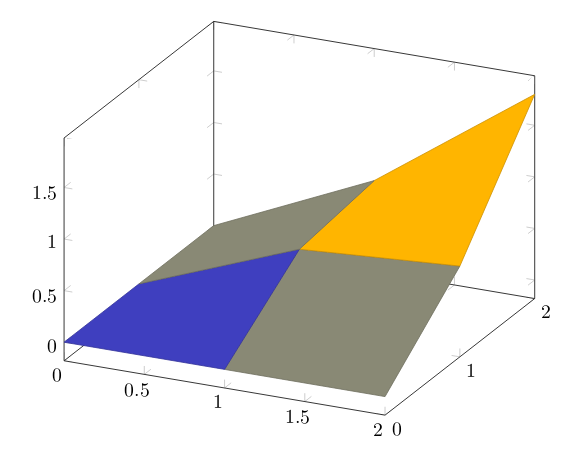
\includegraphics[width=8cm]{Imagenes/Pgfplot3d3}
    \captionof{chart}{Three dimensional graph.}
    \label{cha:chart1}
    \end{chart}
    
    \begin{figure}[h]
    \centering
    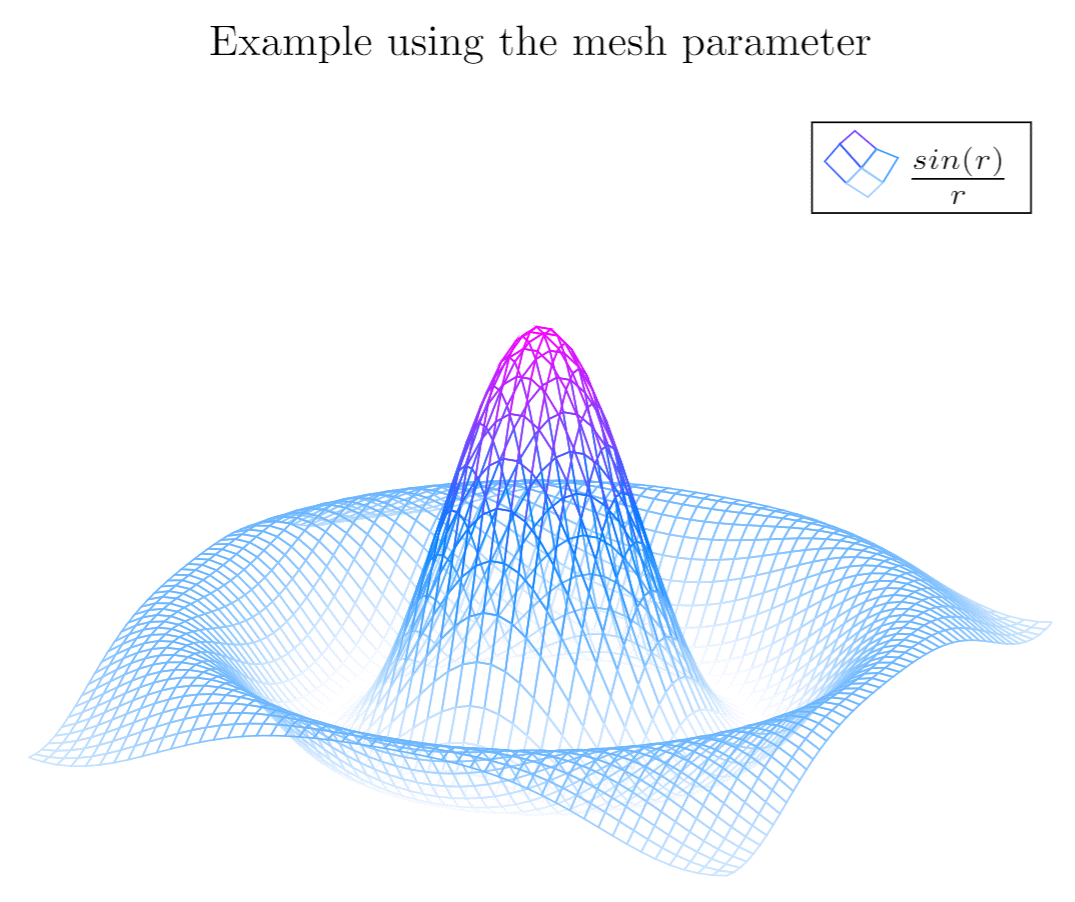
\includegraphics[width=0.5\textwidth]{Imagenes/pgfplots3dexample.png}
    \caption{Second 3D plot.}
    \label{fig:figure1}
    \end{figure}

    \begin{illustration}
        \caption{This is an example caption.}
        \label{ill:blah}  
        \begin{itemize}
          \item Possible illustration
        \end{itemize}
      \end{illustration}
%-------------------------------------------------------------------
\section*{\ProximoCapitulo}
%-------------------------------------------------------------------
\TocProximoCapitulo

...

% Variable local para emacs, para  que encuentre el fichero maestro de
% compilaci�n y funcionen mejor algunas teclas r�pidas de AucTeX
%%%
%%% Local Variables:
%%% mode: latex
%%% TeX-master: "../Tesis.tex"
%%% End:
